\documentclass[11pt]{article}

\input{./preamble.tex}

%%
%% DOCUMENT START
%%

\begin{document}
\fancypagestyle{allpages}
{
	\fancyhf[LH]{}
	\fancyhf[CH]{}
	\fancyhf[RH]{\thepage}
	\fancyhf[LF]{}
	\fancyhf[CF]{}
	\fancyhf[RF]{}
}

\fancypagestyle{firstpage}
{
	\fancyhf[LH]{\Large Final Project \\ \large ASEN 6519: Uncertainty Quantification}
	\fancyhf[CH]{}
	\fancyhf[RH]{\large Ryan Skinner \\ \large Due 2016/5/6}
	\fancyhf[LF]{}
	\fancyhf[CF]{}
	\fancyhf[RF]{}
}

\pagestyle{allpages}
\thispagestyle{firstpage}
\renewcommand{\sectionmark}[1]{ \markright{#1}{} }

\vspace*{0in}
\begin{center}
\Large
Bi-Fidelity Modeling of Geometric Impact on NACA Airfoil Performance
\\[1ex]
\large
Ryan Skinner$^1$
\\[1ex]
\normalsize
$^1$University of Colorado, Boulder, CO USA
\end{center}
\vspace*{0.3in}

\section*{Abstract}
We undertake a bi-fidelity investigation into the effect of geometric and angle of attack design parameters on the performance of a 2-D NACA 4412 airfoil at low-Mach and Reynolds number of 3 million. All simulations rely on the steady Spalart-Allmaras (SA) RANS turbulence closure. Low-fidelity simulations use a coarse mesh with unresolved boundary layers, whereas high-fidelity simulations employ a refined mesh that fully resolves the near-wall BL. Predictive capacity of the bi-fidelity approach is validated with pressure coefficient data.

%%%%%%%%%%%%%%%%%%%%%%%%%%%%%%%%%%%%%%%%%
%%%%%%%%%%%%%%%%%%%%%%%%%%%%%%%%%%%%%%%%%
\section{Introduction}
%%%%%%%%%%%%%%%%%%%%%%%%%%%%%%%%%%%%%%%%%
%%%%%%%%%%%%%%%%%%%%%%%%%%%%%%%%%%%%%%%%%

The need to characterize and optimize the design of unsteady aerodynamic systems becomes more pressing as atmospheric vehicles push performance boundaries. Despite advances over the last five decades in turbulence modeling, capturing the relevant dynamics is prohibitively expensive in the context of design optimization (DO). The finite time to market for most high-performance aerospace products constrains simulations' quantity and rigor, resulting in sub-optimal performance. Any method that accelerates unsteady aerodynamic design is directly applicable to industry, as better-performing systems can reduce fuel expenditures and environmental impact, especially in the commercial aviation sector.

The bi-fidelity approach seeks to address the shortcomings of traditional brute-force DO strategies. The cost associated with accurate simulations of unsteady aerodynamic systems makes it particularly promising in this context. Bi-fidelity modeling consists of two steps. First, a number of low-fidelity (LF) simulations are run. LF simulations do not capture the exact physics of the system, but place low demand on computational resources. These LF realizations are used to generate both an interpolation and a low-rank approximation of a solution quantity as a function of design parameters. LF simulations could employ less stringent numerical convergence criteria, coarser meshes, or less-accurate turbulence models. Second, high-fidelity (HF) simulations are run for each combination of parameters deemed important by the low-rank approximation, and are used in conjunction with the low-fidelity interpolating coefficients to approximate the solution response over the parameter space.

The bi-fidelity DO approach is equally applicable to uncertainty quantification (UQ). Rather than building a specific, optimal design of the NACA airfoil, small variations in geometric design parameters can be used to quantify the impact of manufacturing defects on performance metrics. Coupling DO with UQ, this approach allows for characterization of the chosen optimum's resilience in the presence of manufacturing defects.

Though the 2-D NACA 4412 airfoil used here has little topical interest, it is nonetheless selected for two reasons. First, it is a standard academic geometry that was thoroughly studied in the 1930s and '40s, resulting in readily-available validation data (see NACA reports 563, 613, and 824). Second, applying the bi-fidelity approach to DO of a NACA airfoil offers a proving ground for the method and analysis tools, which can be scaled up to more industrially-relevant systems in future work. Ultimately, this technology will expanded to multi-fidelity simulations of flow over complex engineering geometries, such as a multi-element airfoil at high angle of attack or active flow control in an aggressive subsonic diffuser.

\begin{figure}[ht]
\begin{center}
\includegraphics[width=\textwidth]{naca_mesh_1.png}
\\[1.5ex]
\includegraphics[height=4cm]{naca_mesh_3.png}
\hspace*{1ex}
\includegraphics[height=4cm]{naca_mesh_4.png}
\vspace{1ex}
\caption{106,000-element 2-D mesh of fluid domain around a NACA 4412 airfoil used for preliminary studies. Counter-clockwise from top: full domain, intermediate zoom, high zoom on airfoil.}
\label{fig:mesh}
\end{center}
\end{figure}

%%%%%%%%%%%%%%%%%%%%%%%%%%%%%%%%%%%%%%%%%
%%%%%%%%%%%%%%%%%%%%%%%%%%%%%%%%%%%%%%%%%
\section{Problem Definition}
%%%%%%%%%%%%%%%%%%%%%%%%%%%%%%%%%%%%%%%%%
%%%%%%%%%%%%%%%%%%%%%%%%%%%%%%%%%%%%%%%%%

%%%%%%%%%%%%%%%%%%%%%%%%%%%%%%%%%%%%%%%%%
%%%%%%%%%%%%%%%%%%%%%%%%%%%%%%%%%%%%%%%%%
\section{Implementation}
%%%%%%%%%%%%%%%%%%%%%%%%%%%%%%%%%%%%%%%%%
%%%%%%%%%%%%%%%%%%%%%%%%%%%%%%%%%%%%%%%%%

The shape of a 4-digit NACA xyzz airfoil is specified by three geometric parameters, all non-dimensionalized with respect to the chord length $c$:
\begin{itemize}
\item $m = \text{x} / 100$ is the maximum camber
\item $p = \text{y} / 10$ is the location of maximum camber
\item $t = \text{zz}/100$ is the maximum thickness
\end{itemize}

For a physical coordinate $x \in [0, c]$, the thickness of a symmetric airfoil is given by
\begin{equation}
y_t = 5tc\, \left[ 0.2969 \sqrt{\frac{x}{c}} + (-0.1260) \left(\frac{x}{c}\right) + (-0.3516) \left(\frac{x}{c}\right)^2 + 0.2843 \left(\frac{x}{c}\right)^3 + (-0.1015) \left( \frac{x}{c} \right)^4 \right]
\end{equation}
The coordinate pairs of points on the upper $(x_U, y_U)$ and lower $(x_L, y_L)$ surface are simply $x_U = x_L = x$, $y_U = y_t$, and $y_L = -y_t$. A symmetric airfoil corresponds to the NACA 00zz series. One example is NACA 0012, shown in \figref{fig:naca0012}.

Cambered NACA airfoils define thickness perpendicular to the camber line, which can be defined as
\begin{equation}
y_c = \begin{cases}
m \frac{x}{p^2} \left( 2p-\frac{x}{c}\right) & 0 \le x \le pc \\
m \frac{c-x}{(1-p)^2} \left(1-2p+\frac{x}{c}\right) & pc \le x \le c
\end{cases}
\end{equation}
The upper and lower coordinate pairs become
\begin{equation}
\begin{aligned}
x_U &= x - y_t \sin \theta &\quad y_U &= y_c + y_t \cos \theta \\
x_L &= x + y_t \sin \theta &\quad y_L &= y_c - y_t \cos \theta
\end{aligned}
\end{equation}
where
\begin{equation}
\theta = \arctan \left( \dd{y_c}{x} \right)
\quad \text{and} \quad
\dd{y_c}{x} =
\begin{cases}
\frac{2m}{p^2} \left( p - \frac{x}{c} \right) & 0 \le x \le pc \\
\frac{2m}{(1-p)^2} \left( p - \frac{x}{c} \right) & pc \le x \le c
\end{cases}
\end{equation}

Because cambered profiles are generated from their symmetric counterparts, we can analytically determine the displacements necessary to deform any symmetric NACA mesh into an arbitrary 4-digit NACA mesh. This results in substantial efficiency gains. In our case, we create a CAD model of a NACA 0012 airfoil, mesh it, and partition it once. Then, in the initialization stage of a new simulation, we generate a stochastic NACA realization parameterized by random variables $\mb{m}$, $\mb{p}$, and $\mb{t}$. Each mesh node on the airfoil surface is prescribed a displacement based on its $x$-coordinate, which is then passed to a linear elastic structural solver. Numerical solution of the unsteady incompressible Navier-Stokes equations proceeds on the deformed mesh.

\begin{figure}[b]
\begin{center}
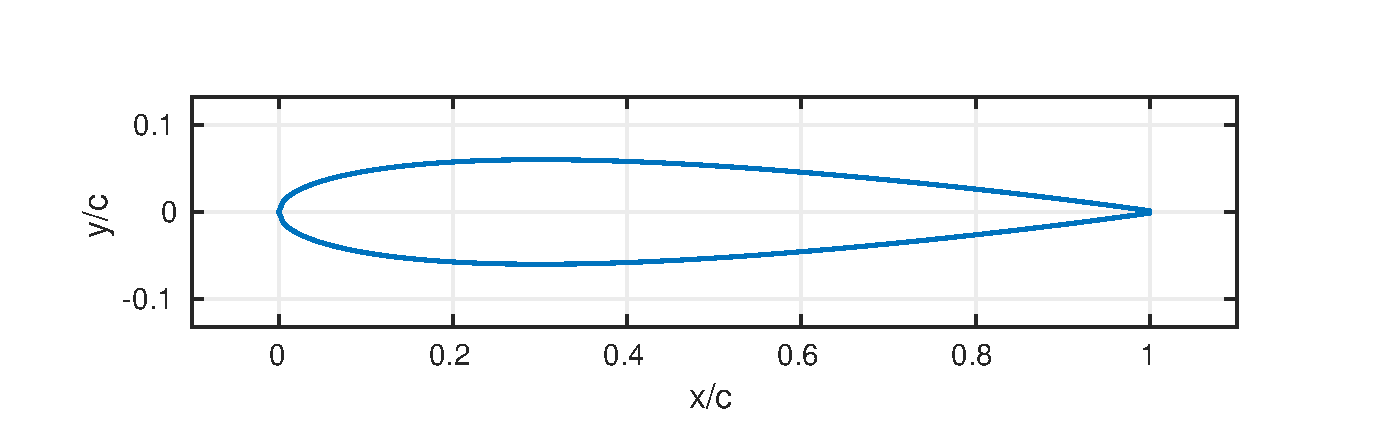
\includegraphics[width=0.85\textwidth]{naca0012.eps}
\vspace{1ex}
\caption{Surface of a NACA 0012 airfoil.}
\label{fig:naca0012}
\end{center}
\end{figure}

\section{Solution Approach}

To quantify the geometry, the following design parameters corresponding to a 4-digit series NACA airfoil are selected: maximum camber $m$, location of maximum camber $p$, maximum thickness $t$, and angle of attack $\alpha$. All but $\alpha$ are specified as a fraction of the chord $c$, which we take to be unity. Performance characteristics of the airfoil are the pressure coefficient distribution $C_p(x)$ and the coefficient of lift $C_L$.

We begin by meshing the fluid volume around a standard NACA 4412 airfoil at zero angle of attack, as shown in Figure \ref{fig:mesh}. This allows us to iterate the mesh until the airfoil curvature is adequately captured. Boundary and initial conditions are defined, and after partitioning the domain to take advantage of solver parallelism, the simulation is run with PHASTA until statistically stationary results are obtained.

This solution acts as the starting point for each new combination of design parameters we want to test. Geometric parameters are specified in an ASCII input file. Upon reading this file, PHASTA applies a displacement to each node on the surface of the airfoil, represented by the black lines in Figure \ref{fig:deform}. A linear elastic structural solver satisfies the displacement constraint and deforms the entire mesh in accordance with the specified geometric parameters. As before, numerical solution of the flow equations proceeds until statistically-steady results are again obtained, or until a given number of time steps have passed. LF simulations use the Spalart-Allmaras (SA) RANS model on a coarse grid.

Each LF simulation uses randomly selected inputs (within the allowed range) for the geometric parameters. When the simulation's stopping criterion is met, $C_p$ and $C_L$ information is extracted from the solution, and stored with a geometric identifier specifying $m$, $p$, $t$, and $\alpha$. For a given set of runs, an interpolating decomposition (ID) is used to determine which geometries contribute most to the variation in performance characteristics (see Doostan et.~al. 2016).

HF simulations are then run for only the select few geometric configurations with the largest ID coefficients. These HF simulations combine SA-RANS with large eddy simulation (LES) through dynamic detached-eddy simulation (DDES). Because they resolve unsteady shedding, the HF runs require time averaging, whereas the low-fidelity RANS simulations do not. The truncated ID is then used to reconstruct the solution quantities of interest: expansion coefficients from the ID of LF-origin are combined with their corresponding basis vectors, which now come from HF simulations.

To verify the accuracy of the bi-fidelity approach, more HF simulations are run using geometric configurations not present in the truncated expansion. The HF simulation results are compared to those predicted by the truncated bi-fidelity expansion.

\section{Results}

The linear elastic mesh deformation code\footnote{Provided by Eric Peters, University of Colorado, Boulder, CO USA} has been fully integrated into PHASTA, in addition to the NACA-specific code to specify essential displacement boundary conditions. At this time, the implementation is still being debugged. The initial NACA 4412 mesh has been generated as well, and automation of $C_L$ and $C_p$ data extraction is underway.

\section{Conclusion and Discussion}

At the time of writing, no conclusions can be drawn as data acquisition and analysis is still in progress.


%\begin{figure}[h]
%\begin{center}
%\includegraphics[width=0.7\textwidth]{example_deformation.eps}
%\vspace{1ex}
%\caption{Deforming an arbitrary body into a NACA airfoil at 30$\degree$ angle of attack. Black lines indicate mapping from blue to red curve.}
%\label{fig:deform}
%\end{center}
%\end{figure}



%%
%% DOCUMENT END
%%
\label{lastpage}
\end{document}



























